\section{Kundenbefragung} \label{sec:befragung}

Um zunächst die Markenpositionierung von Garmin zu ermitteln ist es notwendig eine Kundenbefragung durchzuführen. Mithilfe der Antworten dieser Umfrage ist es möglich einen ungefähren Überblick zur Markenpositionierung von Garmin zu finden. Der Fragebogen und die Antworten sind jeweils im Anhang (\ref{tab:fragebogen}, \ref{tab:kunden}) zu finden. Es sollte jedoch bedacht werden, dass aufgrund der limitierten Anzahl an befragten Personen, nur ein grober Überblick geschafft wird.

\subsection{Top of Mind Awareness}
Die Top of Mind Awareness  ist ein Begriff der Markenbekanntheit und beschreibt welche Marke Personen als erstes für eine bestimmte Kategorie einfällt. Sprich mit welchem Produkt als erstes eine Assoziation zu einer Produktkategorie geknüpft wird. Die Top of Mind Awareness ist ein essentieller Bestandteil bei Kaufentscheidungen von potentiellen Kunden und deshalb auch ein sehr wichtiges Kriterium zur Bewertung der Stärke einer Marke. Die Agreggierung von Neukunden wird durch die Top of Mind Awareness auch viel leichter, da die Marke bei Recherchen bzw. Gesprächen viel schneller in den Vordergrund rückt. Ist die Marke aufgrund von z.B. Skandalen bei vielen Kunden im Kopf, kann die Top of Mind Awareness jedoch auch negativ sein.  \cite{ToMA-1} \cite{ToMA-2}

Anhand der Befragung \ref{sec:befragung} lässt sich leicht feststellen, dass Garmin eine sehr hohe Top of Mind Awaraness bei Sportuhren besitzt, da jeder befragte als erste Marke Garmin aufgezählt hat. In Abbildung \ref{fig:toMa} ist dies nochmals grafisch zu sehen, dabei ist zu beachten, dass manche Personen 2 Marken gewählt haben. 


\begin{figure}[H]
    \centering
    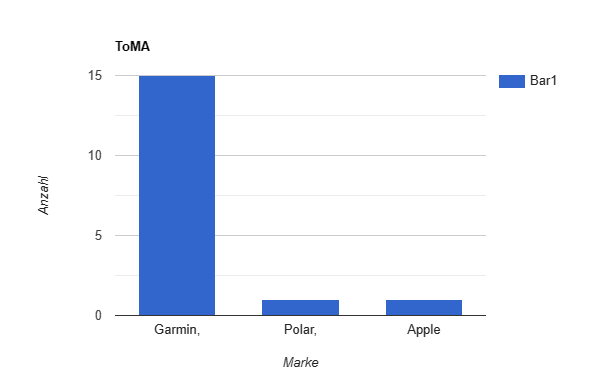
\includegraphics[width=0.7\linewidth]{Figure/ToMA.png}
    \caption{Garmin - Top of Mind Awaraness}
    \label{fig:toMa}
\end{figure}


Es sollten jedoch keine voreiligen Schlüsse gezogen werden, da die befragten Personen bereits alle Garmin Uhren besitzen und im alltäglichen Gebrauch verwenden. Zudem konnten alle Personen noch einige weitere Marken nennen. Um eine genauerer Positionierung zu ermitteln, müsste eine viel größere Anzahl an Personen befragt werden und auch eine weniger homogene Gruppe befragt werden.

\subsection{Involvement}
Bei Marketing spricht man bei Involvement meist bei Entscheidungs- bzw. Kaufsituationen. Involvement beschreibt grundlegend wie viel Zeit und Energie Kunden in die Suche und Bewertung von Produkten investieren. Dabei lassen sich Käufe grob in zwei Kategorien einteilen.
\begin{itemize}
    \item \textbf{High-Involvement:} Die Kaufentscheidung wird durch eine intensive Recherche und viele Vergleiche zwischen verschiedenen Produkten getätigt. Dabei handelt es sich bei High-Involvement Käufen meist um eher teurere Anschaffungen, wie z.B. eine Uhr oder ein Auto. In der High-Involvement Kategorie spielt die stärke einer Marke eine essentielle Rolle damit der Kunde ein Gefühl von Sicherheit erhält. Damit sind diese Käufe auch stark mit der Top of Mind Awareness verknüpft.
    \item \textbf{Low-Involvement:}
    Die Kaufentscheidung wird meist unterbewusst und ohne lange Recherche getätigt. Dabei handelt es sich meist um eher billigere Produkte, wie z.B. Waschmittel. Die stärke einer Marke ist hier nicht unbedingt ausschlaggebend. \cite{Involvement-1} \cite{Involvement-2}
\end{itemize}

Sportuhren fallen aufgrund des nicht so geringen Preis eher in die Kategorie von High-Involvement Gegenständen. Das ist auch bei Garmin Uhren so und ist anhand der Befragung \ref{sec:befragung} sehr einfach ersichtlich. Nahezu alle befragten haben vor dem Kauf der Uhr recherchiert und vergleiche zwischen verschiedenen Marken durchgeführt bevor es zu einem Kauf gekommen ist. In den Abbildungen (\ref{fig:inv1}, \ref{fig:inv2}) ist zu sehen ob sich die Befragten zuvor informiert haben und auch ob sie das Produkt Online oder im Geschäft gekauft haben.

\begin{figure}[!h]
  \centering
  \begin{minipage}[b]{0.48\textwidth}
    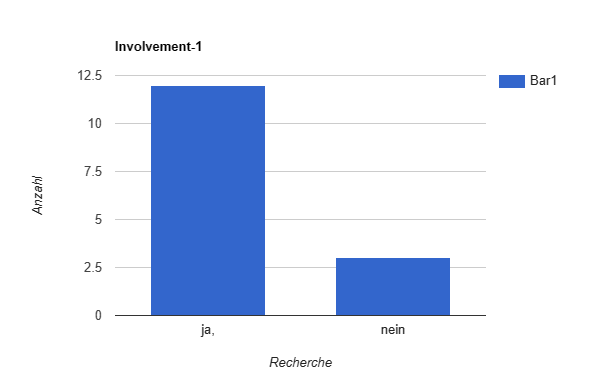
\includegraphics[width=\textwidth]{Figure/involvement-1.png}
      \caption{Garmin - Involvement}
    \label{fig:inv1}
  \end{minipage}
  \hfill
  \begin{minipage}[b]{0.48\textwidth}
    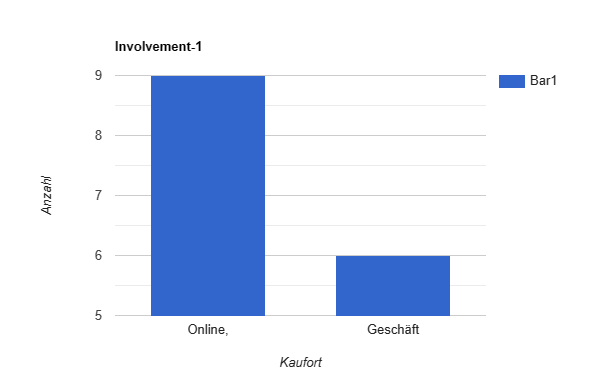
\includegraphics[width=\textwidth]{Figure/involvement-2.png}
    \caption{Garmin - Kaufort}
    \label{fig:inv2}
  \end{minipage}
\end{figure}




\newpage


% Luki
\subsection{Bewertungskriterien}
Die Befragten stützen sich auf verschiedene Merkmalen beim Vergleich von Garmin mit anderen Marken. Einige der hervorgehobenen Merkmale sind die Funktionsvielfalt, Genauigkeit der Daten, Benutzerfreundlichkeit der Geräte, und die Optik der Uhren. Im Zuge dieser Umfrage wurde auch schnell klar, dass sich Garmin bereits einen starken Namen in der gesamten Sport Gemeinschaft gemacht hat und alleine durch Image und Mundpropaganda einen großen Kundenkreis schafft. 

In Bezug auf den Nutzen, den Garmin-Produkte für die Befragten schaffen, wurde eine Reihe von Aspekten hervorgehoben. Dazu gehören die Unterstützung vieler verschiedener Sportarten, die Qualität der Trainingsdaten und bereitgestellten Metriken sowie die Robustheit und Akkulaufzeit der Geräte. Diese Aspekte deuten auf einen hohen funktionalen Nutzen hin. Darüber hinaus scheint Garmin auch einen emotionalen Nutzen zu bieten, da die Befragten ihre Geräte sowohl beim Sport als auch im Alltag als ständigen Begleiter dabei haben.

\subsection{Wettbewerbsvorteile}
Die Befragten nehmen Garmin in Bezug auf mehrere kaufentscheidende Merkmale als höherwertig wahr als seine Konkurrenten. Insbesondere wurde die Software und das soziale Netzwerk von Garmin sowie der Funktionsumfang und die Metriken als Unterscheidungsmerkmale hervorgehoben. Darüber hinaus wurde die große Auswahl an Modellen, die Funktionsvielfalt und die Robustheit der Garmin-Produkte als Wettbewerbsvorteile angesehen.

Es ist auch bemerkenswert, dass die Befragten Garmin als Anbieter von hochwertigen Produkten wahrnehmen. Dies deutet darauf hin, dass die Marke in Bezug auf die Produktqualität einen starken Wettbewerbsvorteil hat. Schließlich wurde die Fähigkeit von Garmin, viele Metriken über den Fortschritt zu liefern, als ein weiteres Unterscheidungsmerkmal genannt, das Garmin von seinen Konkurrenten abhebt.

Zusammenfassend lässt sich sagen, dass die Befragten Garmin in Bezug auf eine Reihe von Merkmalen positiv bewerten und die Marke als wertvoll für ihre sportlichen und alltäglichen Aktivitäten ansehen. Dies deutet darauf hin, dass Garmin eine starke Position im Markt für Sport- und Outdooruhren hat.


\newpage


% Mathias
\subsection{Markenimage}
Das Markenimage bezieht sich auf die Wahrnehmung und Vorstellung die Kunden von einem Unternehmen besitzen. Es bildet sich aus verschiedenen Komponenten wie Werbung, Produkterfahrung und der wahrgenommenen Qualität. Dabei führt ein positives Markenimage zu einer hohen Kundenloyalität und stärkt die Marktposition eines Unternehmens.\cite{Markenimage}  
Anhand der Antworten in der Kundenbefragung ist eine klare Tendenz erkennbar, denn die Kunden assoziieren die Produkte der Marke Garmin vor allem mit folgenden Eigenschaften:
\begin{itemize}
    \item Robustheit
    \item Genauigkeit
    \item Funktionsvielfalt
    \item Kompatibilität
\end{itemize} 
Dies führt dazu, dass die Marke im Allgemeinen sehr positiv wahrgenommen wird. Dies deckt sich auch mit den Antworten bezüglich dem Wettbewerbsvorteil, denn auch hier geben die Befragten meist Antworten die sich auf die Qualität der Garmin Produkte beziehen.
Man kann also festhalten, dass sich Garmin seinen Stärken bewusst ist und diese gezielt nutzt, da diese den Kunden beeindrucken und den Kundennutzen darstellen und somit das Markenimage bilden. Denn die positiven Erlebnisse die der Kunde mit den Produkten von Garmin hat, ergeben schlussendlich das Markenimage. Dies deckt sich auch mit den Ergebnissen bezüglich der ungestützen Markenbekanntheit. Hier haben die Befragten stets Garmin genannt, was von einer großen Bekanntheit zeugt, was wiederum die Vorraussetzung für ein gutes Markenimage bildet. 

\subsection{Net Promoter Score (NPS)}

Der Net Promoter Score (NPS) wird verwendet, um die Loyalität und Zufriedenheit von Kunden mit einem Unternehmen zu messen.Um dies messen zu können wird eine einfache Frage gestellt: "Wie wahrscheinlich ist es das sie Ihr Garmin Gerät weiterempfehlen würden? (1: unwahrscheinlich; 10: sehr wahrscheinlich)". Anschließend werden die Kunden je nach Antwort eingestuft, wobei es drei Kategorien von Kunden gibt:
\begin{itemize}
    \item Promotoren (9-10)
    \item Passive (7-8)
    \item Kritiker (0-6)
\end{itemize}
Die Anzahl der Kritiker in Prozent wird dann von der Anzahl der Promotoren in Prozent abgezogen und das Ergebnis ist dann der Net Promoter Score. Das Ergebnis der Kundenberfragung zu Garmin ergibt einen NPS von circa 67. Dieses Ergebnis ist in Abbildung \ref{fig:NPS} veranschaulicht. Es ist zu erkennen, dass es keine Kritiker gibt, das heißt es waren alle Kunden zufrieden. Der NPS ist sehr hoch, was für eine sehr hohe Kundenzufriedenheit spricht, und beweist die Kundenorientierung des Unternehmens. \cite{Netigate-NPS} 

\begin{figure}[h]
	\centering
	\begin{tikzpicture}
    \pie[pos ={8,0},
    radius=2,
    text=legend,
    color={cyan,blue}]
    {33.3 / Passive , 66.7 / Promoter} 
    \end{tikzpicture}
    \vspace{0.5cm}
	\caption{Garmin - Net Promoter Score}
    \label{fig:NPS}
\end{figure}

Diesen sehr guten NPS nutzt Garmin indem die gesamte Produktpalette unter einer Marke verkauft und beworben wird, wie in Kapitel \ref{Markenarchitektur} beschrieben. Dies gibt dem Unternehmen die Möglichkeit, die positiven Kundenerfahrungen und somit auch das Markenimage von einem Produkt auf das nächste zu übertragen. 

